\begin{table}[!t]
\caption{Distinct USWNs and associated sets of \unravelled traces from a single Sepsis Cases Event Log \cite{mannhardt_2016}.}\label{tab:dataset}
 \begin{adjustbox}{max width=\textwidth}
	\begin{tabular}{crl||cl|c}
		\toprule
		\textbf{Experiment Conf.} $(\mathcal{U})$ & \textit{Model} & $+$\textit{W. Estimator} & $n$ & $p_\theta$& $\;\;|\mathcal{W}_{p_\theta}^n(P_{\mathcal{U}})|$ \\
		\midrule
		
		\textbf{SM\_CONS\_20} &SplitMiner 2.0  \cite{AugustoCDRP19}       & +\texttt{Constant} & $20$ & $\;\;0$ & $157$  \\
		
		\textbf{SM\_FORK\_20} & SplitMiner 2.0  \cite{AugustoCDRP19}      & +Fork \cite{spdwe} & $20$ & $\;\;0$ & $32$  \\
		
		
		\textbf{SM\_PAIR\_20} & SplitMiner 2.0  \cite{AugustoCDRP19}      & +PairScale \cite{spdwe} & $20$ & $\;\;0$ & $157$ \\
		
		\textbf{SM\_PETRI\_20} & \multicolumn{2}{c||}{Rogge-Solti \cite{RoggeSoltiAW13}} & $20$ & $10^{-5}$ & $1612$ \\
		\bottomrule
	\end{tabular}
\end{adjustbox}
\end{table}
\section{Experimental Results}\label{sec:exp}
\subsection{Dataset}
For our experiments, we took the Sepsis Cases event log \cite{mannhardt_2016} and split the dataset into a training set, containing the ``\textit{happy traces}''  having duration lower than or equal to the average trace duration in the log ($\leq 2.3\cdot 10^{7}$ ms), and a test set, containing the traces with the highest execution times. We used the training set to generate either a USWN, using the approach presented in \cite{RoggeSoltiAW13}, or a BPMN with only exclusive gates using Split Miner 2.0 \cite{AugustoCDRP19} that was then converted into a Petri net \cite{PPNFromLog}. This Petri net was later on converted into a USWN by using a firing weight estimator: we choose the Fork and the PairScale estimators from \cite{spdwe} and we denote as \texttt{Constant} a naive estimator assuming that all the transition enabled in a given marking are equiprobable. %No estimator was used for the USWN generated via ProM, as such engine already estimates the firing weights.
From such USWNs, we generated distinct sets of \unravelled\ traces. All these steps are summarised in \tablename~\ref{tab:dataset}. The following experiments have the aim of evaluating the benefits of performing the Approximate-Ranking strategy over the Optimal-Ranking one.

\begin{figure*}[!t]
\begin{minipage}{.49\textwidth}

	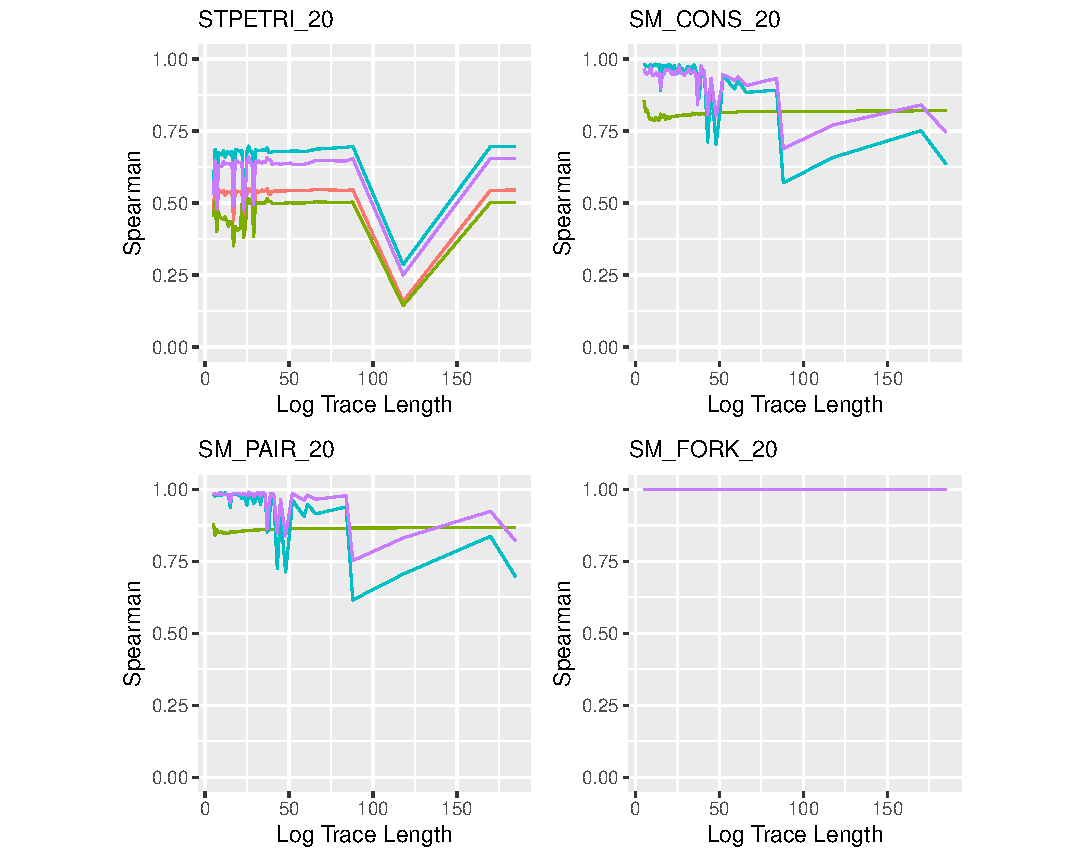
\includegraphics[width=1.1\textwidth]{images/Prec.pdf}
	\caption{Approximation comparison.}\label{fig:app}
\end{minipage}\hfill \begin{minipage}{.49\textwidth}

	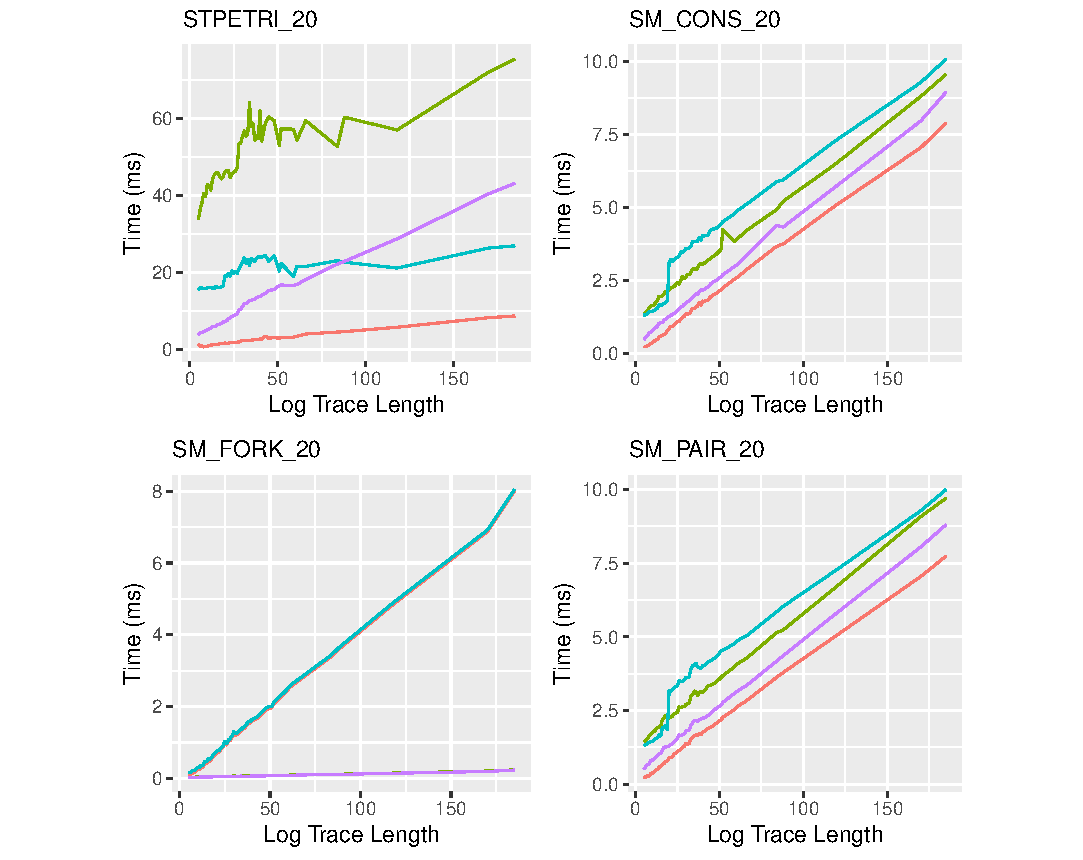
\includegraphics[width=1.1\textwidth]{images/kronos.pdf}
	\caption{$k$NN alignment benchmark.}\label{fig:kronos}
\end{minipage}
\end{figure*}
\subsection{Approximation}\label{subsec:apprp}
In order to assess how well the proposed Approximate-Ranking strategy approximates the Optimal-Ranking one, we use the Spearman correlation index \cite{SCI} to express the correlation between each sub-embedding strategies for $\phi_{\mathcal{P}}$ ($\color{ggplotGreen}\epsilon^1\&\nu^1$, $\color{ggplotRed}\epsilon^2\&\nu^1$, $\color{ggplotPurple}\epsilon^1\&\nu^2$, and $\color{ggplotBlue}\epsilon^2\&\nu^2$) and the Optimal-Ranking. In \figurename~\ref{fig:app}, we show the average Spearman index for traces of different lengths in the test set.
We can see from the plots that the sub-embeddings considering only information about the edges (i.e., the ones where the features corresponding to the $\nu$ dimension are set to zero) have in general a higher correlation with the Optimal-Ranking strategy, but their correlation values are less stable with respect to the length of the trace to be aligned. In the case of \textbf{SM\_PETRI\_20}, the correlation is lower than for the other configurations (lower than 0.7 for all sub-embeddings). For \textbf{SM\_PAIR\_20} and \textbf{SM\_CONS\_20}, the correlation index is around 0.8 for $\color{ggplotPurple}\epsilon^1\&\nu^2$ and $\color{ggplotBlue}\epsilon^2\&\nu^2$, and almost 1 for $\color{ggplotGreen}\epsilon^1\&\nu^1$ and $\color{ggplotRed}\epsilon^2\&\nu^1$ but less stable for these sub-embeddings especially for longer traces. In the case of \textbf{SM\_FORK\_20}, the correlation is maximum for all sub-embedding strategies.

%set of \unravelled traces in Table \ref{tab:dataset} and the subset of the Sepsis Cases Event Log that was not used to generate the USWNs. For each of this log trace $\sigma^*$ we added controlled noise (transition addition, deletion, or swap) at either $20\%$ ($\tilde{\sigma}^*$) or $30\%$ ($\tilde{\tilde{{\sigma}}}^*$) of the log trace as for \cite{LeoniM17}. Then, we found the correlation between the ranking $R_\star$ induced by $k_{\phi_{\mathcal{P}}}(\sigma,\sigma^*)$ to the ranking induced by replacing $\sigma^*$ with one of the two noised traces (either a ranking $R_{20}$ induced by $k_{\phi_{\mathcal{P}}}(\sigma,\tilde{\sigma}^*)$ or $R_{30}$ induced by $k_{\phi_{\mathcal{P}}}(\sigma,\tilde{\tilde{\sigma}}^*)$). The correlation $\rho$ between these two rankings ($\rho(R_\star,R_{20})$ and $\rho(R_\star,R_{30})$) is performed via Spearman Correlation Index $\rho$: such index will return near-$1$ on increasing monotonic trend, near-$(-1)$ values on decreasing monotonic trend, and near-$0$ values where the two rankings are almost uncorrelated. Figure \ref{fig:app} shows the outcome of such experiments for all the possible combinations of $\epsilon$ and $\nu$ sub-embeddings for $\phi_{\mathcal{P}}$ while varying the log trace length. We can observe that strategies including traces' frequencies ($\nu^1$) are more stable if compared to strategies where such information is completely ignored ($\nu^2$). Furthermore, such approximation never reaches zero values, while that occurrence might happen for $\nu^2$-based strategies.

\subsection{Efficiency}\label{subsec:efficio}
With reference to the plots in \figurename~\ref{fig:kronos}, we evaluated the efficiency of computing the trace alignment over both Optimal-({\color{ggplotPurple}Purple} and {\color{ggplotGreen}Green}) and Approximate-Ranking ({\color{ggplotBlue}Blue} and {\color{ggplotRed}Red}) strategies over two different data structures enabling $k$NN queries, i.e., VP-Trees ({\color{ggplotBlue}Blue} and {\color{ggplotPurple}Purple}) and KD-Trees ({\color{ggplotRed}Red} and {\color{ggplotGreen}Green}). We conduct our experiments for $k=20$\ADD{, and we use the Levenshtein distance as distance function}. While the query time for the Optimal-Ranking includes the \textit{indexing time} for generating every time all the vectors of the search space and the time for the neighbourhood search, the Approximate-Ranking includes the neighbourhood search time and the time neede for the embedding transformation of the trace to be aligned $x$; in particular, we consider the average embedding time for all the possible embedding strategies described in the experimental setting escribed in the previous section. \figurename~\ref{fig:kronos} plots the result of such experiments: the time required to generate and load all the $\phi_\star$ truly dominates the cost of generating the embedding $\phi_{\mathcal{P}}(x)$ for bigger datasets such as \textbf{SM\_PETRI\_20}, while the cost for $\phi_{\mathcal{P}}(x)$ becomes non-negligible when we have just a few traces to align (\textbf{SM\_FORK\_20}). 
%Last, while the $k$NN alignments over $\phi_{\mathcal{P}}$ always provide the best timing results via KD-Trees, we cannot elect a best data structure $\phi_\star$ that is valid for all datasets and all trace lengths. 